\documentclass[../../main.tex]{subfiles}
\begin{document}
\chapter{浅层神经网络}
% Shallow neural networks

\section{神经网络概述}
% Neural Network Overview

\section{神经网络的表示}
% Neural Network Representation

\section{计算一个神经网络的输出}
% Computing a Neural Network's output

\section{多样本向量化}
% Vectorizing across multiple examples

\section{向量化实现的解释}
% Justification for vectorized implementation

\section{激活函数}
% Activation functions
在隐藏层和输出层,先进行一个\textbf{线性变换}:\(z^{[1]}=W^{[1]}x + b^{[1]}\),然后再进行一个非线性变换,也就是经过\textbf{非线性激活函数},计算出该节点的\textbf{输出值}(激活值)。

激活函数必须有且必须是非线性函数,假如某一层使用了\textbf{线性激活函数}(恒等激活函数),或者没有使用激活函数,可以看出输出值都是线性组合后的值(都进行了线性变换),而下一层也肯定会先进行线性变换,那么这层没有什么意义;假如所有的激活函数都是线性函数,那么最终的输出结果仍然是原始输入的线性组合,无论网络规模有多大,都相当于单层的线性回归。\\
\begin{remark}
    线性激活函数可能在一些特殊情况有应用。
\end{remark}


常见的激活函数有四种:\textbf{sigmoid}、\textbf{tanh}、\textbf{ReLU}、\textbf{Softmax},另外还有两种 ReLU 函数的变体:\textbf{Leaky ReLU}、\textbf{Parametric ReLU}。\\
\begin{remark}
    sigmoid意思是S形,sigmoid函数叫做 \textbf{logistic} 更准确
\end{remark}

\subsection{sigmoid}
逻辑回归教程中首先介绍的就是sigmoid函数,可以将取值\(-∞, +∞\)的数映射到\((0, 1)\)之间。
\[σ(z) = \frac{1}{1+e^{-z}}\]
\begin{figure}[H]
    \centering
    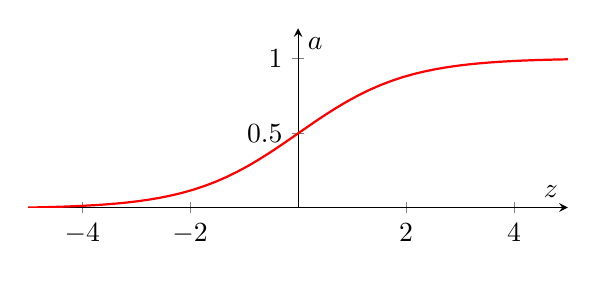
\begin{tikzpicture}
    \begin{axis}[
        axis y line = center,
        axis x line = middle,
        y post scale = 0.4,
        ytick = {0.5, 1},
        ymax = 1.2,
        xlabel=\(z\),
        ylabel={\(a\)}
    ]
    \addplot[color=red,thick,samples=50]{1/(1+exp(-x))};
    \end{axis}
\end{tikzpicture}
\end{figure}
求导:
\begin{align*}
    σ'(z) & = (\frac{1}{1+e^{-z}})'       \\
          & = \frac{e^{-z}}{(1+e^{-z})^2} \\
          & = σ(z)(1- σ(z))
\end{align*}
sigmoid并不常用,因为具有不少缺点:
\begin{enumerate}
    \item 计算麻烦。
    \item 当 \(z\) 值非常大或者非常小时,使得梯度更新十分缓慢,即\textbf{梯度消失}。
    \item 输出不是以0为均值,不便于下层的计算。
\end{enumerate}
所以sigmoid一般仅用于二分类的输出层。

\subsection{tanh}
tanh函数在数学上,时sigmoid函数拉伸、平移后的结果,它取值\(-∞, +∞\)的数映射到\((-1, 1)\)之间。
\[\tanh(z) = \frac{e^{z}-e^{-z}}{e^{z}+e^{-z}}\]
\begin{figure}[H]
    \centering
    \begin{tikzpicture}
    \begin{axis}[
        axis y line = center,
        axis x line = middle,
        y post scale = 0.8,
        ytick = {-1,-0.5,0,0.5, 1},
        ymax = 1.2,
        ymin = -1.2,
        xlabel=\(z\),
        ylabel={\(a\)}
    ]
    \addplot[color=red,thick,samples=100]{(exp(x)-exp(-x))/(exp(x)+exp(-x))};
    \end{axis}
\end{tikzpicture}
\end{figure}
求导:
\begin{align*}
    g'(z) & = (\frac{e^{z}-e^{-z}}{e^{z}+e^{-z}})' \\
          & = \frac{4}{(e^{z}+e^{-z})^2}           \\
          & = 1-g^2(z)
\end{align*}
相比sigmoid,tanh,均值为0,利于下一层计算,但仍然具有\(z\) 值非常大或者非常小时,梯度消失的问题,相较于sigmoid也要更常用一些。

\subsection{ReLU}
ReLU函数又称为\textbf{修正线性单元(Rectified Linear Unit)},是一种分段线性函数,弥补了sigmoid函数以及tanh函数的梯度消失问题。
\[g(z) = \max(0, z)\]
\begin{figure}[H]
        \centering
        \begin{tikzpicture}
        \begin{axis}[
            axis y line = center,
            axis x line = middle,
            y post scale = 0.5,
            xlabel=\(z\),
            ylabel={\(a\)},
            domain=-2:2,
        ]
        \addplot[red,thick]{(x>=0)*x};
        \end{axis}
    \end{tikzpicture}
\end{figure}
求导:\[g'(z) = \begin{cases}
    1 & , z>0 \\
    0 & ,z<0
\end{cases}\]
ReLU函数的优点:
\begin{enumerate}
    \item 计算简单。
    \item 当\(z>0\)时,不存在梯度消失问题。
\end{enumerate}
缺点则是当\(z<0\)时,梯度为0,梯度消失。
\subsubsection{Leaky ReLU}
Leaky ReLU是ReLU的改进版本,当输入值是负值时,函数值不等于0,而是给了一个很小的负数梯度值\(α\)。这个函数通常比 ReLU 激活函数效果要好,但是效果不是很稳定,所以在实际中Leaky ReLU使用的并不多。
\[g(z) = \max{(α×z,z)}\]
\begin{figure}[H]
    \centering
    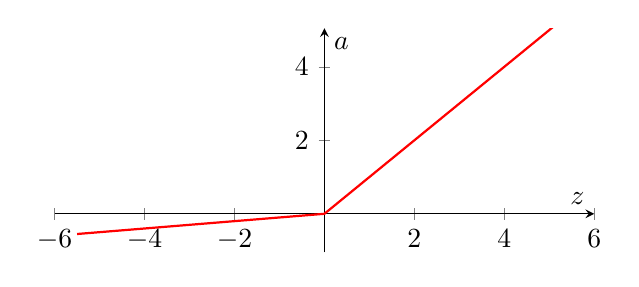
\begin{tikzpicture}
        \begin{axis}[
            axis lines=middle,
            xmax=6,
            xmin=-6,
            ymin=-1.05,
            ymax=5.05,
            y post scale = 0.5,
            xlabel={$z$},
            ylabel={$a$}]
        \addplot [domain=-5.5:5.5, thick, red] {max(0.1 * x, x)};
        \end{axis}
    \end{tikzpicture}
\end{figure}
\subsubsection{Parametric ReLU}
相比Leaky ReLU将负输入的梯度设为超参数,Parametric ReLU将\(α\)作为一个可学习的参数,会在训练的过程中进行更新。

\subsection{Softmax}
% TODO Softmax 函数写在这里
\[
    g(z_i) = \frac{e^{z_i}}{\sum\limits_{j=0}^n{e^{z_i}}}
\]

\section{为什么需要非线性激活函数?}
% why need a nonlinear activation function?

\section{激活函数的导数}
% Derivatives of activation functions

\section{神经网络的梯度下降}
% Gradient descent for neural networks

\section{直观理解反向传播}
% Backpropagation intuition

\section{随机初始化}
% Random Initialization
\end{document}